\section{Survival of small populations}
\label{sec:small}

Quasi-stationarity describes what a surviving population looks like once it has survived
for a long time. The complementary question is how it gets there from a small founding
number, and near criticality the answer is dominated by the first few generations. This
section works through that early regime, records the discrete birth--death--catastrophe
calculation that later chapters build on, and then computes the continuous-time
counterpart of $A(p)$, where a closed form is available and the comparison is
informative.

\subsection{The first few generations}
\label{sec:firstgens}

Take the binary process near criticality, so that division and death each have
probability close to a half. A founding lineage then dies at its very first round almost
half the time. Should it pass that round, its two offspring must each fail at their own
first attempt for the lineage to end there, which happens with probability about
$0.25$; so the lineage reaches the second generation with probability roughly
\begin{equation*}
0.375 \approx
\underbrace{(1-0.5)}_{\text{no extinction at the first step}}
\times
\underbrace{(1-0.5\times0.5)}_{\text{nor at the second}} .
\end{equation*}
Iterating \cref{eq:unIter,eq:SnIter} from $u_0=0$, $S_0=1$ makes this exact. At precise
criticality the first four values are
\begin{equation*}
u_n = 0.500,\ 0.625,\ 0.695,\ 0.741 \qquad(3\ \text{s.f.},\ n=1,2,3,4),
\end{equation*}
so survival decays quickly over the first few rounds of replication, and it does so
almost as fast just above criticality as just below (\cref{fig:earlySn}). Whatever
advantage supercriticality confers, it is not an early-generation advantage: the curves
for $p=0.45$, $0.5$ and $0.55$ have barely separated by $n=4$, and nearly all of the
extinction risk has already been spent.

\begin{figure}[ht]
\centering
  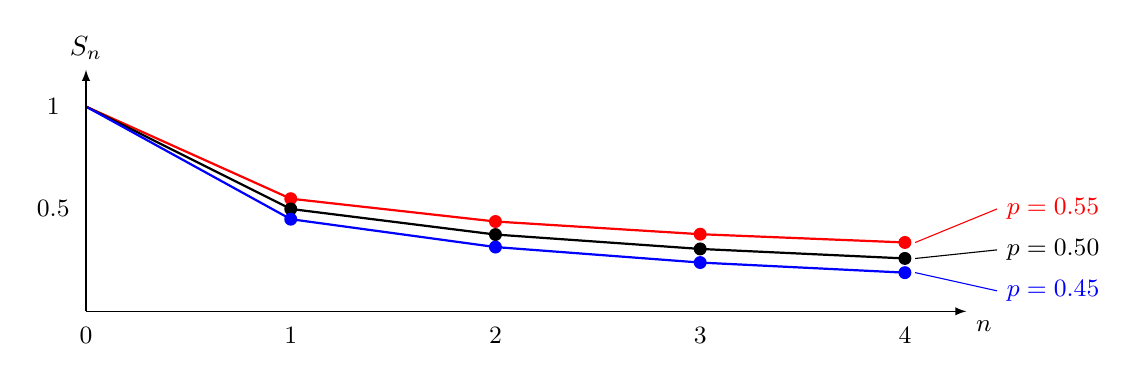
\begin{tikzpicture}[scale = 2.6]
    \foreach \x/\y/\color in {1/0.55/red, 2/0.4386250/red, 3/0.3766719/red, 4/0.336304/red,
                              1/0.5/black, 2/0.375/black, 3/0.3046875/black, 4/0.25827/black,
                              1/0.449999/blue, 2/0.313874/blue, 3/0.2381546/blue, 4/0.188816/blue}
      \fill[color=\color] (\x, \y) circle (0.9pt);
    \draw[red, thick] (0, 1) -- (1, 0.55) -- (2, 0.4386250) -- (3,0.3766719) -- (4,0.336304);
    \draw[black, thick] (0, 1)--(1,0.5) --  (2,0.375) -- (3,0.304687) -- (4,0.25827);
    \draw[blue, thick] (0, 1)--(1,0.449999)  --  (2,0.313874) -- (3,0.238154) -- (4,0.18881);
    \draw[-latex] (0,0) -- (4.3,0) node[below right, font=\small] {$n$};
    \draw[-latex] (0,0) -- (0,1.18) node[above] {$S_n$};
    \foreach \x/\lab in {0/0, 1/1, 2/2, 3/3, 4/4} \node[font=\small] at (\x, -0.12) {\lab};
    \foreach \y/\lab in {0.5/0.5, 1/1} \node[font=\small] at (-0.16, \y) {\lab};
    \draw[red,  thin] (4.05,0.336) -- (4.45,0.50);
    \draw[black,thin] (4.05,0.258) -- (4.45,0.30);
    \draw[blue, thin] (4.05,0.189) -- (4.45,0.10);
    \node[red,  font=\small, anchor=west] at (4.45, 0.50) {$p=0.55$};
    \node[black,font=\small, anchor=west] at (4.45, 0.30) {$p=0.50$};
    \node[blue, font=\small, anchor=west] at (4.45, 0.10) {$p=0.45$};
  \end{tikzpicture}
\caption{Survival probability over the first four generations from a single progenitor,
obtained by iterating \cref{eq:SnIter}. The decay is steep even in the supercritical case
$p=0.55$, and the three curves remain close together throughout. The difference between
sub- and supercriticality is a difference in late behaviour, not in early risk.}
\label{fig:earlySn}
\end{figure}

\subsection{An initial cohort of size \texorpdfstring{$k$}{k}}
\label{sec:cohort}

Now let the process begin with $\zz_0=k$ individuals rather than one --- a group small to
moderate in number, perhaps $k=10$. Under supercritical branching, growth becomes more
predictably exponential as the count rises, because a large population lets the expected
dynamics show through the noise of individual events. A founding cohort is precisely the
regime in which that noise still dominates.

The persistence of such a cohort is a question about its lineages. All $k$ founders
branch independently, so the population is extinct at generation $n$ exactly when every
one of the $k$ lineages has died out by then, each with probability $u_n$. Hence
\begin{equation}
\label{eq:Snk}
S^{(k)}_n = 1-\bigl(u_n\bigr)^{k},
\end{equation}
which is \cref{eq:pgfindep} in its most elementary form. \Cref{fig1,fig2} plot
$S^{(k)}_n$ out to $500$ generations for $k=1,10,100,1000$.

\begin{figure}[ht]
\centering
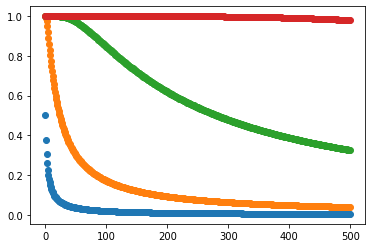
\includegraphics[width=0.56\textwidth]{figures/IMG_ch3/kvals.png}
\caption{Survival probability $S^{(k)}_n$ from \cref{eq:Snk} out to $500$ generations at
exact criticality, $p=0.5$, for $k=1,10,100,1000$ (blue through to red). A larger
founding cohort buys longevity, but at criticality every curve is still headed for zero.}
\label{fig1}
\end{figure}

\begin{figure}[ht]
\centering
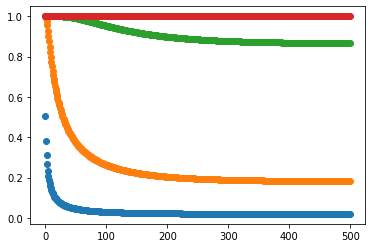
\includegraphics[width=0.45\textwidth]{figures/IMG_ch3/kvals505.png}
\hfill
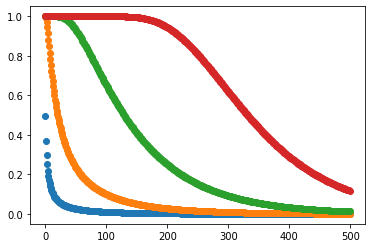
\includegraphics[width=0.45\textwidth]{figures/IMG_ch3/kvals495.png}
\caption{As \cref{fig1}, but with $p$ displaced slightly from criticality: $p=0.505$ on
the left (supercritical) and $p=0.495$ on the right (subcritical). The benefit of a large
founding cohort is acutely sensitive to which side of $\tfrac12$ the process sits on. A
displacement of half a per cent separates curves that were nearly coincident in
\cref{fig1}.}
\label{fig2}
\end{figure}

The effect visible in \cref{fig1} --- that a larger first cohort gives improved longevity
--- is thus strongly modulated by criticality. Persistence improves rapidly as $p$
approaches $\tfrac12$ from below, and continues to improve dramatically into
supercriticality, where a large $k$ converts a modest per-lineage survival probability
into near-certain establishment. What a founding cohort buys, in other words, depends
almost entirely on a parameter it does not itself control.

\subsection{An aside on early replication}
\label{sec:earlyrep}

The same conditioning effect has been identified in a setting far from the present one:
the longevity and diversity of phylogenetic clades. Clades that have persisted through
the ages, and which are often the more diverse, turn out to have experienced an
above-average early rate of species origination --- an observation drawn from the fossil
record itself. Budd and Mann \cite{Budd2018} argue that this empirical pattern may be a
statistical consequence rather than a biological one. Run a large number of homogeneous
birth--death processes, retain only those that happen to survive to some arbitrary large
time --- \enquote{the present} --- and the retained set is automatically enriched for
early rapid origination, with no change in the underlying rates required. The apparent
slowdown in diversification that follows is then not a slowdown at all but a reversion to
the mean, an effect known as the \emph{push of the past}.

That is the conditioning of \cref{sec:qsd} seen from the other side. There we conditioned
a subcritical process on survival and found its mean settling at $1/A(p)$ instead of
decaying; here one conditions a critical or supercritical process on survival to the
present and finds its early growth inflated. In both cases the conditioning, not the
mechanism, does the work, and in both cases the effect is largest where the survival
probability is smallest.

The parallel suggests a modelling hypothesis worth carrying forward: that early
replication may strongly affect eventual survival probabilities even when later
per-capita rates are unchanged. \Cref{fig:earlySn} is the reason to take it seriously,
since the first few generations are where nearly all of the extinction risk is
concentrated.

\subsection{Discrete birth--death--catastrophe}
\label{sec:bdc}

Later chapters replace the pure birth--death mechanism by one in which the whole
population can be eliminated at a stroke. It is worth recording here what that addition
does in discrete time, since the answer is partly inherited from the Galton--Watson
analysis above.

Up to the moment of catastrophe, a discrete-time birth--death--catastrophe process
behaves exactly as the basic Galton--Watson model as far as its limiting conditional
distribution is concerned. Conditioning on non-rupture, and conditioning also on
non-extinction by death, the process exhibits a stationary limiting distribution of the
kind derived in \cref{sec:qsd}. Whether a quasi-stationary distribution survives when one
conditions on \emph{neither} death nor catastrophe is a separate question, and one best
settled by simulation. Either way it is useful to have the probability of non-catastrophe
in hand.

\subsubsection*{Rupture at step \texorpdfstring{$n$}{n}}

Let $\kappa$ be the probability that a given individual initiates catastrophe at a given
step. A single individual fails to cause rupture with probability $1-\kappa$, two with
$(1-\kappa)^2$, and a cohort of size $N$ with $(1-\kappa)^N$.

Take first the case of birth and catastrophe only, with no death. The census is then
known with certainty at every generation: from a single progenitor the population simply
doubles at each step prior to catastrophe. The process therefore comes to its abrupt halt
in generation $n$ with probability
\begin{equation}
\label{eq:bdcrupture}
1-(1-\kappa)^{2^{\,n-1}},
\end{equation}
one minus the probability that none of the $2^{n-1}$ individuals present caused it.

\subsubsection*{Survival of the process}

Along the same lines, and still without death, let $S_n$ be the probability that the
process survives to generation $n$. Survival to generation $0$ is certain, $S_0=1$.
Survival to generation $1$ requires only that the founder replicated without rupture,
$S_1 = 1-\kappa$. Persistence to step $2$ requires that the founder divided and that each
of its two offspring did likewise, so $S_2 = (1-\kappa)(1-\kappa)^2$. Every prior step
must be passed, and the exponents form a geometric series:
\begin{equation}
\label{eq:bdcS}
S_n = \prod_{i=0}^{n-1}(1-\kappa)^{2^i}
= (1-\kappa)^{\sum_{i=0}^{n-1}2^i}
= (1-\kappa)^{2^n-1} .
\end{equation}
Survival therefore fails doubly exponentially in $n$, which is a much more severe
constraint than the geometric decay of \cref{eq:lateS}: with catastrophe present the
population's own growth is what destroys it.

\subsubsection*{Death included}

The difficulty appears as soon as death is allowed, because the size of the living
population is then no longer known with certainty from one generation to the next. The
natural guess is that the probabilities somehow shake out when the expected population is
used in place of the actual one,
\begin{equation}
\label{eq:bdcguess}
S_n \overset{?}{=} (1-\kappa)^{\sum_{i=0}^{n-1}\mean{\zz_i}} ,
\end{equation}
and it is worth being explicit about why \cref{eq:bdcguess} is almost certainly not an
identity. The map $N\mapsto(1-\kappa)^N$ is convex, so Jensen's inequality gives
$\mean{(1-\kappa)^{\zz_i}}\ge(1-\kappa)^{\mean{\zz_i}}$: replacing the random census by
its mean systematically underestimates the chance of getting through a step. Nor are the
steps independent, since surviving one is evidence of a smaller population, which raises
the chance of surviving the next. Both effects push the same way, so \cref{eq:bdcguess}
is better read as a lower bound than as an equality. How tight a bound it is remains a
numerical question, and the exact treatment --- through the rates, the master equation
and its generating function, as in \cref{sec:tools} --- is developed in later chapters for
birth--death--catastrophe processes in continuous time.

\subsection{Continuous-time birth--death}
\label{sec:cts}

The discrete process resists a closed form for $A(p)$, as \cref{sec:Ap} shows at length.
Its continuous-time counterpart does not, and the comparison between the two turns out to
be informative, so we record the continuous-time constant here.

Everything needed is already in \cref{sec:lbd}. For the linear birth--death process with
per-capita rates $\lambda$ and $\mu$ started from $N$ individuals, the extinction
probability is $p_0(t)$ of \cref{eq:p0t} and the survival probability is
$S^{(N)}(t) = 1-p_0(t)$. Exactly as in \cref{sec:condmean}, conditioning on survival gives
\begin{equation}
\label{eq:ctscondit}
\mean{\xt\mid\xt>0} = \frac{\mean{\xt}}{S^{(N)}(t)},
\end{equation}
and the late-time limit follows for any $N$ on applying L'H\^opital's rule. It is quicker
to take $N=1$ and compute directly. With $\mean{\xt} = \ee^{(\lambda-\mu)t}$ from
\cref{eq:lbdmean} and
\begin{equation*}
S(t) = 1-\frac{\mu-\mu\ee^{(\mu-\lambda)t}}{\lambda-\mu\ee^{(\mu-\lambda)t}}
= \frac{\lambda-\mu}{\lambda-\mu\ee^{(\mu-\lambda)t}},
\end{equation*}
equation \cref{eq:ctscondit} gives
\begin{equation*}
\mean{\xt\mid\xt>0} = \frac{\lambda\ee^{(\lambda-\mu)t}-\mu}{\lambda-\mu} .
\end{equation*}
For $\mu>\lambda$ the exponential decays and the limiting conditional mean is a constant,
\begin{equation}
\label{eq:ctsqsmean}
\lim_{t\to\infty}\mean{\xt\mid\xt>0} = \frac{\mu}{\mu-\lambda} = \frac{1}{1-\lambda/\mu}
\;\lrb{= \frac{1}{A_{\text{c}}}} .
\end{equation}
So the subcritical birth--death process is quasi-stationary in the same sense as the
subcritical Galton--Watson process, and with the same structure: a conditional mean that
is the reciprocal of a constant. To compare the two we need a common parameter. An
individual's next event is a division with probability $p = \lambda/(\lambda+\mu)$ by the
race \cref{eq:racen}, so that $\lambda/\mu = p/(1-p)$ and
\begin{equation}
\label{eq:Acts}
\frac{1}{A_{\text{c}}} = \frac{1-p}{1-2p},
\qquad\text{that is}\qquad
A_{\text{c}}(p) = \frac{1-2p}{1-p} .
\end{equation}
The subscript marks this as the continuous-time constant, to be distinguished throughout
from the discrete-time $A(p)$ of \cref{eq:lateS}.

\begin{figure}[ht]
\centering
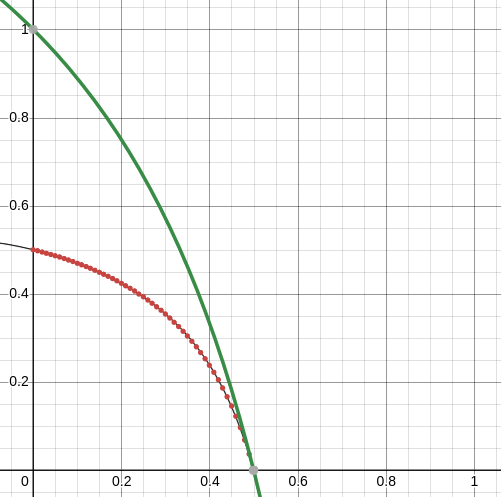
\includegraphics[width=0.5\textwidth]{figures/IMG_ch3/dtctA.png}
\caption{The continuous-time constant $A_{\text{c}}(p) = (1-2p)/(1-p)$ (green) against
high-precision numerical values of the discrete-time constant $A(p)$ (red points). Both
vanish at $p=\tfrac12$, but at $p=0$ the continuous curve starts at $1$ and the discrete
one at $\tfrac12$, and no constant factor relates them in between. The black line is a
formula obtained by symbolic regression (\cref{sec:GA}); it tracks the points closely but
is not exact. \Cref{sec:compare} accounts for the discrepancy exactly.}
\label{fig:dtct}
\end{figure}

\Cref{fig:dtct} plots $A_{\text{c}}(p)$ against numerically computed values of $A(p)$ and
raises an obvious question. Why does the continuous curve start at $1$ where the discrete
one starts at $\tfrac12$, and why does halving $A_{\text{c}}$ not superpose them, given
that at the other end of the range they meet? The answer needs machinery that
\cref{sec:Ap} has still to build; it is given in \cref{sec:compare}, and it turns out that
$A_{\text{c}}(p)/2$ is an exact lower bound for $A(p)$, attained only in the limit
$p\to0$.

\FloatBarrier
